
\documentclass[12pt,a4paper]{scrreprt}
\usepackage[top=1in, bottom=1.25in, left=1.25in, right=1.25in]{geometry}
\usepackage[pdftex]{graphicx}
\usepackage[utf8]{inputenc}
\usepackage[usenames,dvipsnames,svgnames,table]{xcolor}
\usepackage[toc,page]{appendix}
\usepackage[ final ]{pdfpages}
\usepackage{hyperref}
\usepackage[T1]{fontenc}
\usepackage{lmodern}
\usepackage{url}

\def\code#1{\texttt{#1}}

\author{Jeroen Vennegoor op Nijhuis}
\title{E27radio \\ development report}

\begin{document}

\maketitle

\begin{abstract}
Online project archive: 

\begin{itemize}
	\item \url{https://github.com/jevontech/e27radio-image}\\
	\item \url{https://github.com/jevontech/e27radio}\\

\end{itemize}

\begin{center}
\textcopyright 2015 Jeroen Vennegoor op Nijhuis
\end{center}


\end{abstract}

\tableofcontents

\chapter{Introduction}


\section{What is E27radio}
E27radio is a device that makes internet radio accessible to everybody. It enables people from around the world to listen to music and news from many countries around the world. The E27 radio is extremely simple to use once it has been configured properly, so it can be used by anybody, no matter age or education. 

\section{Background}
E27radio was developed as an entry for the Elektor Edison Challenge (end of 2015). I wanted to improve my software development skills for this type of devices, that's why I decided to take part in this competition.
My idea was to use the Intel Edison to build a basic internet radio.
Th initial plan was to use a external DAC(Digital to Analalog converter) in order to create an "analog out" signal that could be input for any audio amplifier.
I ordered a Audio Codec Board from MikroElektronika. It connects to the Intel Edison using I2C for configuration and I2S for the data. 
Direclt from the start I ran into problems trying to use the I2C and I2s bus.
I don't own a logic analyzer, so it was really difficult to see what was actually going wrong on the I2C bus. I gave up after a few weeks...

\begin{figure}[h]
	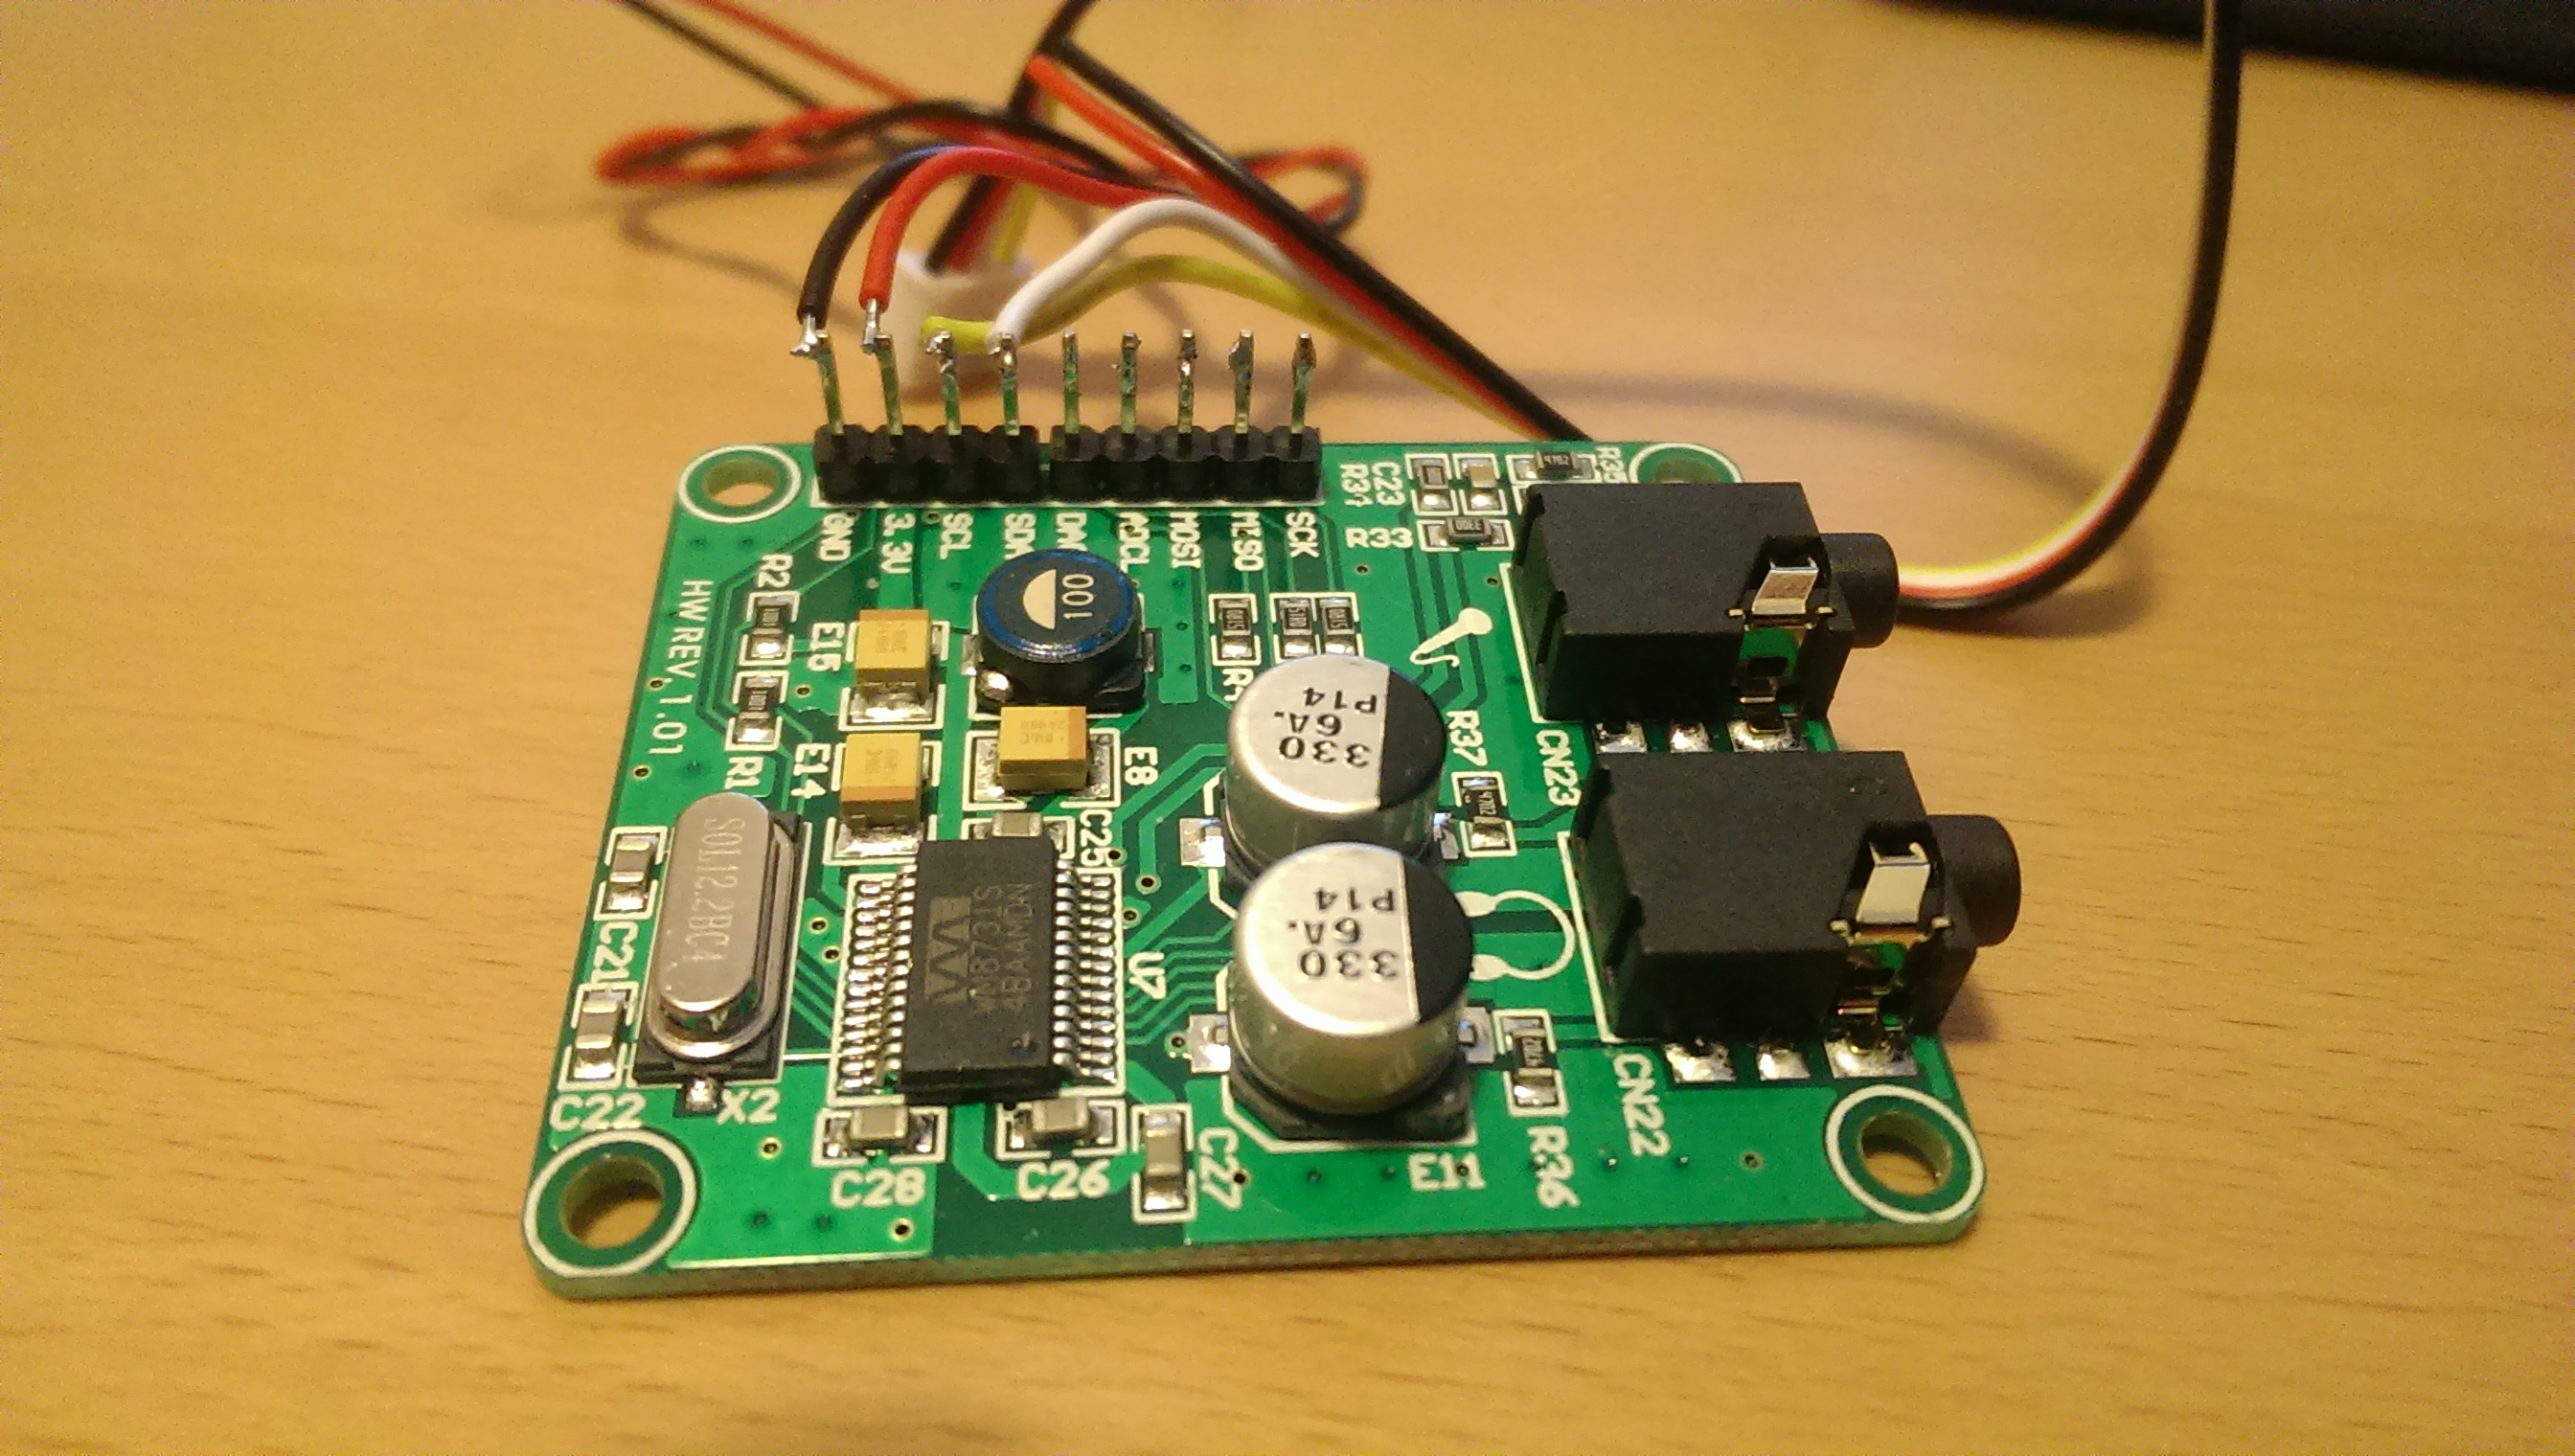
\includegraphics[width=400px]{images/audio1}
	\caption{Audio Codec Board}
\end{figure}

I then decided to take a step back and rethink the whole project.
As the Intel Edison features both WLAN and Bluetooth, I might as well use both in this project. 
So I decided to build an internet radio that actually streams to a Bluetooth speaker. This introduced a lot of new challenges , as you can read in the rest of this report.


\chapter{Design and development}


\section{System architecture}
E27radio is build on the Intel Edison platform.
It uses the onboard Wifi to connect to the Internet , so it can connect to Internet radio stations around the world. Audio output is provided by connecting via Bluetooth to an external speaker.
The user interface consists of a small LCD and a number of push buttons

The application software runs on Yocto Linux (the default for Intel Edison) and is developed in C++.

\begin{figure}[h]
	\includegraphics[height=400px]{images/architecture}
	\caption{System architecture}
\end{figure}


\section{Software overview}
In order to play audio streams via Bluetooth to external speakers, several software functionalities are required.

First of all we need to be able to connect to an Internet radio stream and decode it. This requires a audio player that is able to decode  most common Internet radio audio streams (e.g. MP3). For this I chose "mpg123" (\url{http://mpg123.org/}). Another set of tools is required to actually push this audio stream to a Bluetooth speaker. 
After some research on the Internet, I decided to go for a setup using PulseAudio.
For the actual Bluetooth setup and configuration, a Bluetooth stack is required. For Linux, this is Bluez (\url{http://www.bluez.org/}). 
Bluez is an open source project and exists for quite some time already, but it has almost zero documentation and even less example code. So, that will be a challenge !

\section{Feasibility assessment}

I did a small test with shell scripts and commandline tools to assess whether it is possible to play an audio stream from the Internet to a Bluetooth device using the  Intel Edison.
For this project I am using a JBL portable Bluetooth speaker.

\begin{figure}[h]
	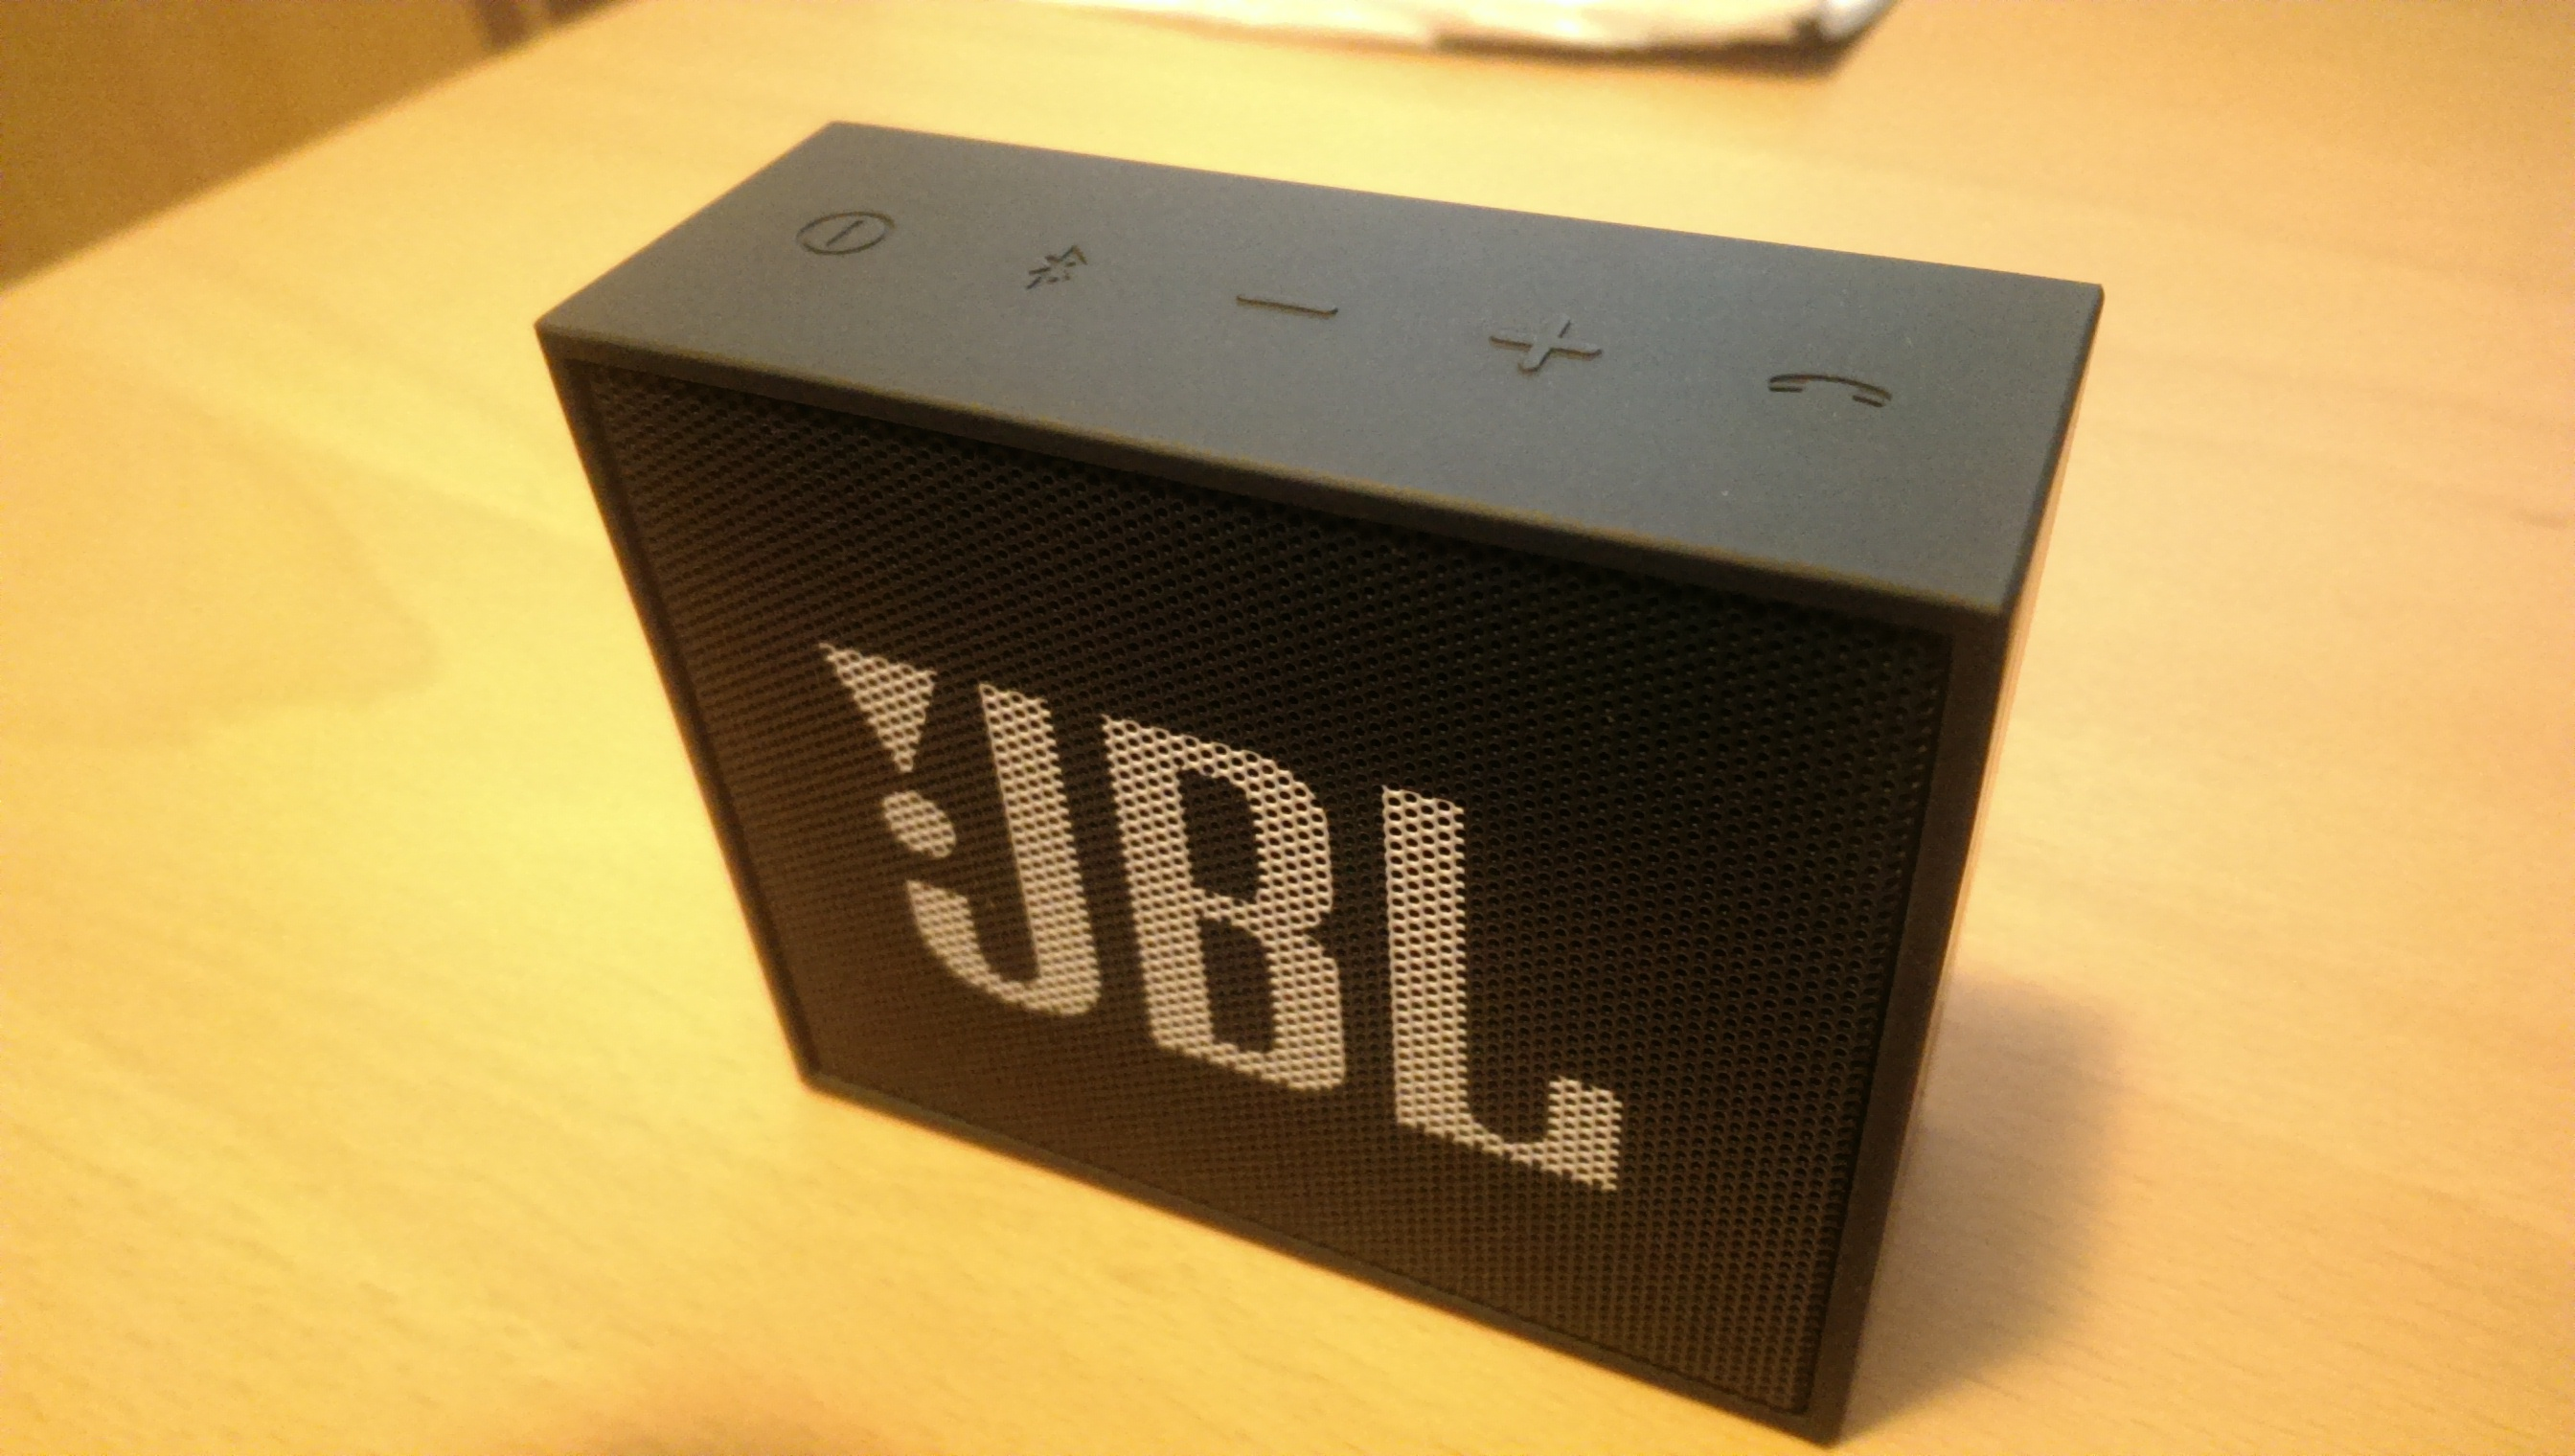
\includegraphics[height=300px]{images/speaker}
	\caption{Bluetooth speaker}
\end{figure}

In order to play  audio, I decided to use 'mpg123' . Unfortunately this software is not available in the official Intel Edison opkg repository. There is an unofficial Intel Edison repository by AlexT (\url{http://alextgalileo.altervista.org/}) and this does include 'mpg123'. But unfortunately this software is build to use Alsa as the default audio sink and not Pulse. 

Thus I decided to set up my own BitBake environment. 
I downloaded the Intel Edison image source from the Intel Edison website and followed the instructions to build the default edison image on my Linux Ubuntu 14.04 PC. 
The initial bitbake takes a lot of time (it builds everything from source) and a LOT of space ( you will need several GigaBytes). 
Once this toolchain worked, I added the recipe for 'mpg123' to the bitbake configuration and I made sure that 'mpg123' uses Pulse audio as default and not Alsa. I could then create a new image for the Edison and flash it on to the board. Once the new image was running on the Intel edison, I configured the Intel Edison to connect to my local WiFi network.(see the Intel Edison website for more information). But we are not done yet: we still need to connect the Intel Edison to the Bluetooth speaker.

Let's go through the manual Bluetooth configuration step-by-step:

\begin{itemize}
	\item Log in to the Intel Edison
	\item Enable the Bluetooth interface: 
	\begin{verbatim}
rfkill unblock bluetooth
	\end{verbatim}
		\item Open the bluetooth agent command line tool:
			\begin{verbatim}
			bluetoothctl
			\end{verbatim}
			\item Enable scanning for Bluetooth devices
			\begin{verbatim}
			scan on
			\end{verbatim}
			\item Pair the Intel Edison with the Bluetooth speaker:
			\begin{verbatim}
		pair xx:xx:xx:xx (the address of the discovered BT speaker)
			\end{verbatim}
				\item Connect to the Bluetooth audio device:
				\begin{verbatim}
				connect xx:xx:xx:xx 
				\end{verbatim}
					\item Quit the Bluetooth agent
					\begin{verbatim}
					quit
					\end{verbatim}	
\end{itemize}

If everything went fine, the audio device you just connected also created an "audio sink" in Pulse audio. We now need to select the sink for this Bluetooth audio device as the "default" audio sink for Pulse audio.

Let's first find it by using:
	\begin{verbatim}
	pactl list | grep bluez_sink
	\end{verbatim}
Look for a name that looks like:
	\begin{verbatim}
	bluez_sink.XX_XX_XX_XX_XX_XX_XX
	\end{verbatim}


Now we need to set that sink as the default:
	\begin{verbatim}
	pactl set-default-sink bluez_sink.XX_XX_XX_XX_XX_XX_XX 
	\end{verbatim}

Now we can select an audio stream from the Internet and play it :
	\begin{verbatim}
mpg123  http://pub1.radiotunes.com:80/radiotunes_tophits
	\end{verbatim}

This works, so the idea of playing audio via Bluetooth with a Intel Edison is feasible.

\section{Software development}
I decided to use my Linux PC for the software development for this project, because I already use it for "BitBaking" the Edison image.
I first used bitbake to create a development toolchain for Linux 64bit. This toolchain is required to cross-compile the software for the Intel Edison platform.
Cmake (\url{http://cmake.org/}) will be used as the build tool for this project , as I have used it before and I am somewhat familiar with it.
Cmake has the advantage that I don't need to write makefiles by hand and it should be fairly easy to switch between crosscompiling using the toolchain and building the software using bitbake.
I created a "toolchain file" that provides cmake with all the information to generate Makefiles that use the compilers for the Intel Edison platform(cross compilation). 

\subsection{Audio playback}
Because mpg123 seemed to work quite well in the feasibility phase I will use mpg123 in the E27-radio software as well. mpg123 includes a C library that can be used by other projects, but I was not quite sure how to use it.
I found some ispiration online (\url{http://hzqtc.github.io/2012/05/play-mp3-with-libmpg123-and-libao.html}) and decided to go for a similar approach with curl, libmpg123 and libao. 
Curl downloads the data, libmpg123 decodes it and then libao plays it.
But I do need to some extra bits and pieces... 
The audio playback needs to run in a seperate thread in order to keep the user interface responsive when audio plackback has started. Stopping the playback was not so trivial, but it can be done by adjusting the return value in the  callback function that curl is calling.  


\subsection{I got the Bluez}
The software for E27radio needs to be able to connect the Intel Edison to a Bluetooth speaker, similar to what we did earlier using the 'bluetoothctl' tool.
In order to do this, the E27radio software needs to 'talk' to the Bluez Bluetooth stack. 
This was one of the hardest parts of the project, as there is almost no information or example code available. 
As far as I could tell, Bluez5 uses only D-Bus for it's API, so I needed to learn how to use D-Bus as well.
D-bus is a message bus system for IPC and RPC. It should be cross-platform, but it is currently only used on Linux, as far as I could tell.
I started looking for any D-Bus library that had a nice clean C++ API, but most D-Bus libraries are a bit outdated and C based (for example libdbus).
I then found out that Qt also has a D-Bus library. The interface seemed nice and clean, so decided to use Qt. 
Qt is normally used for applications that have a graphical user interface, but it should be possible to use it for "embedded applications" as well.

In order to use Qt5 in my project, I needed to include Qt5 in the bitbake project for Intel Edison. For this I started with the Qt5 bitbake layer from the OpenEmbedded project (https://github.com/meta-qt5/meta-qt5 ). I had to make some changes to the configuration in order to force that no GUI related stuff for Qt5 would be build and then I was able to successfully compile Qt5 for my Intel Edison image. 

The Pulse audio sink also needs to be configured, so I created a small class that finds the 'bluez\_sink' and sets it as the default sink. This shouldn't be required if the Bluetooth device has been used before, but I'll do it anyway. In this class I just call an external executable (pactl) , because this was the fastest way to get it working.

\subsection{User interface}
The user interface for this project is very simple: it consists of
\begin{itemize}
	\item 3 push butttons (start/stop, up, down)
	\item Simple LCD display 
\end{itemize}

\begin{figure}[h]
	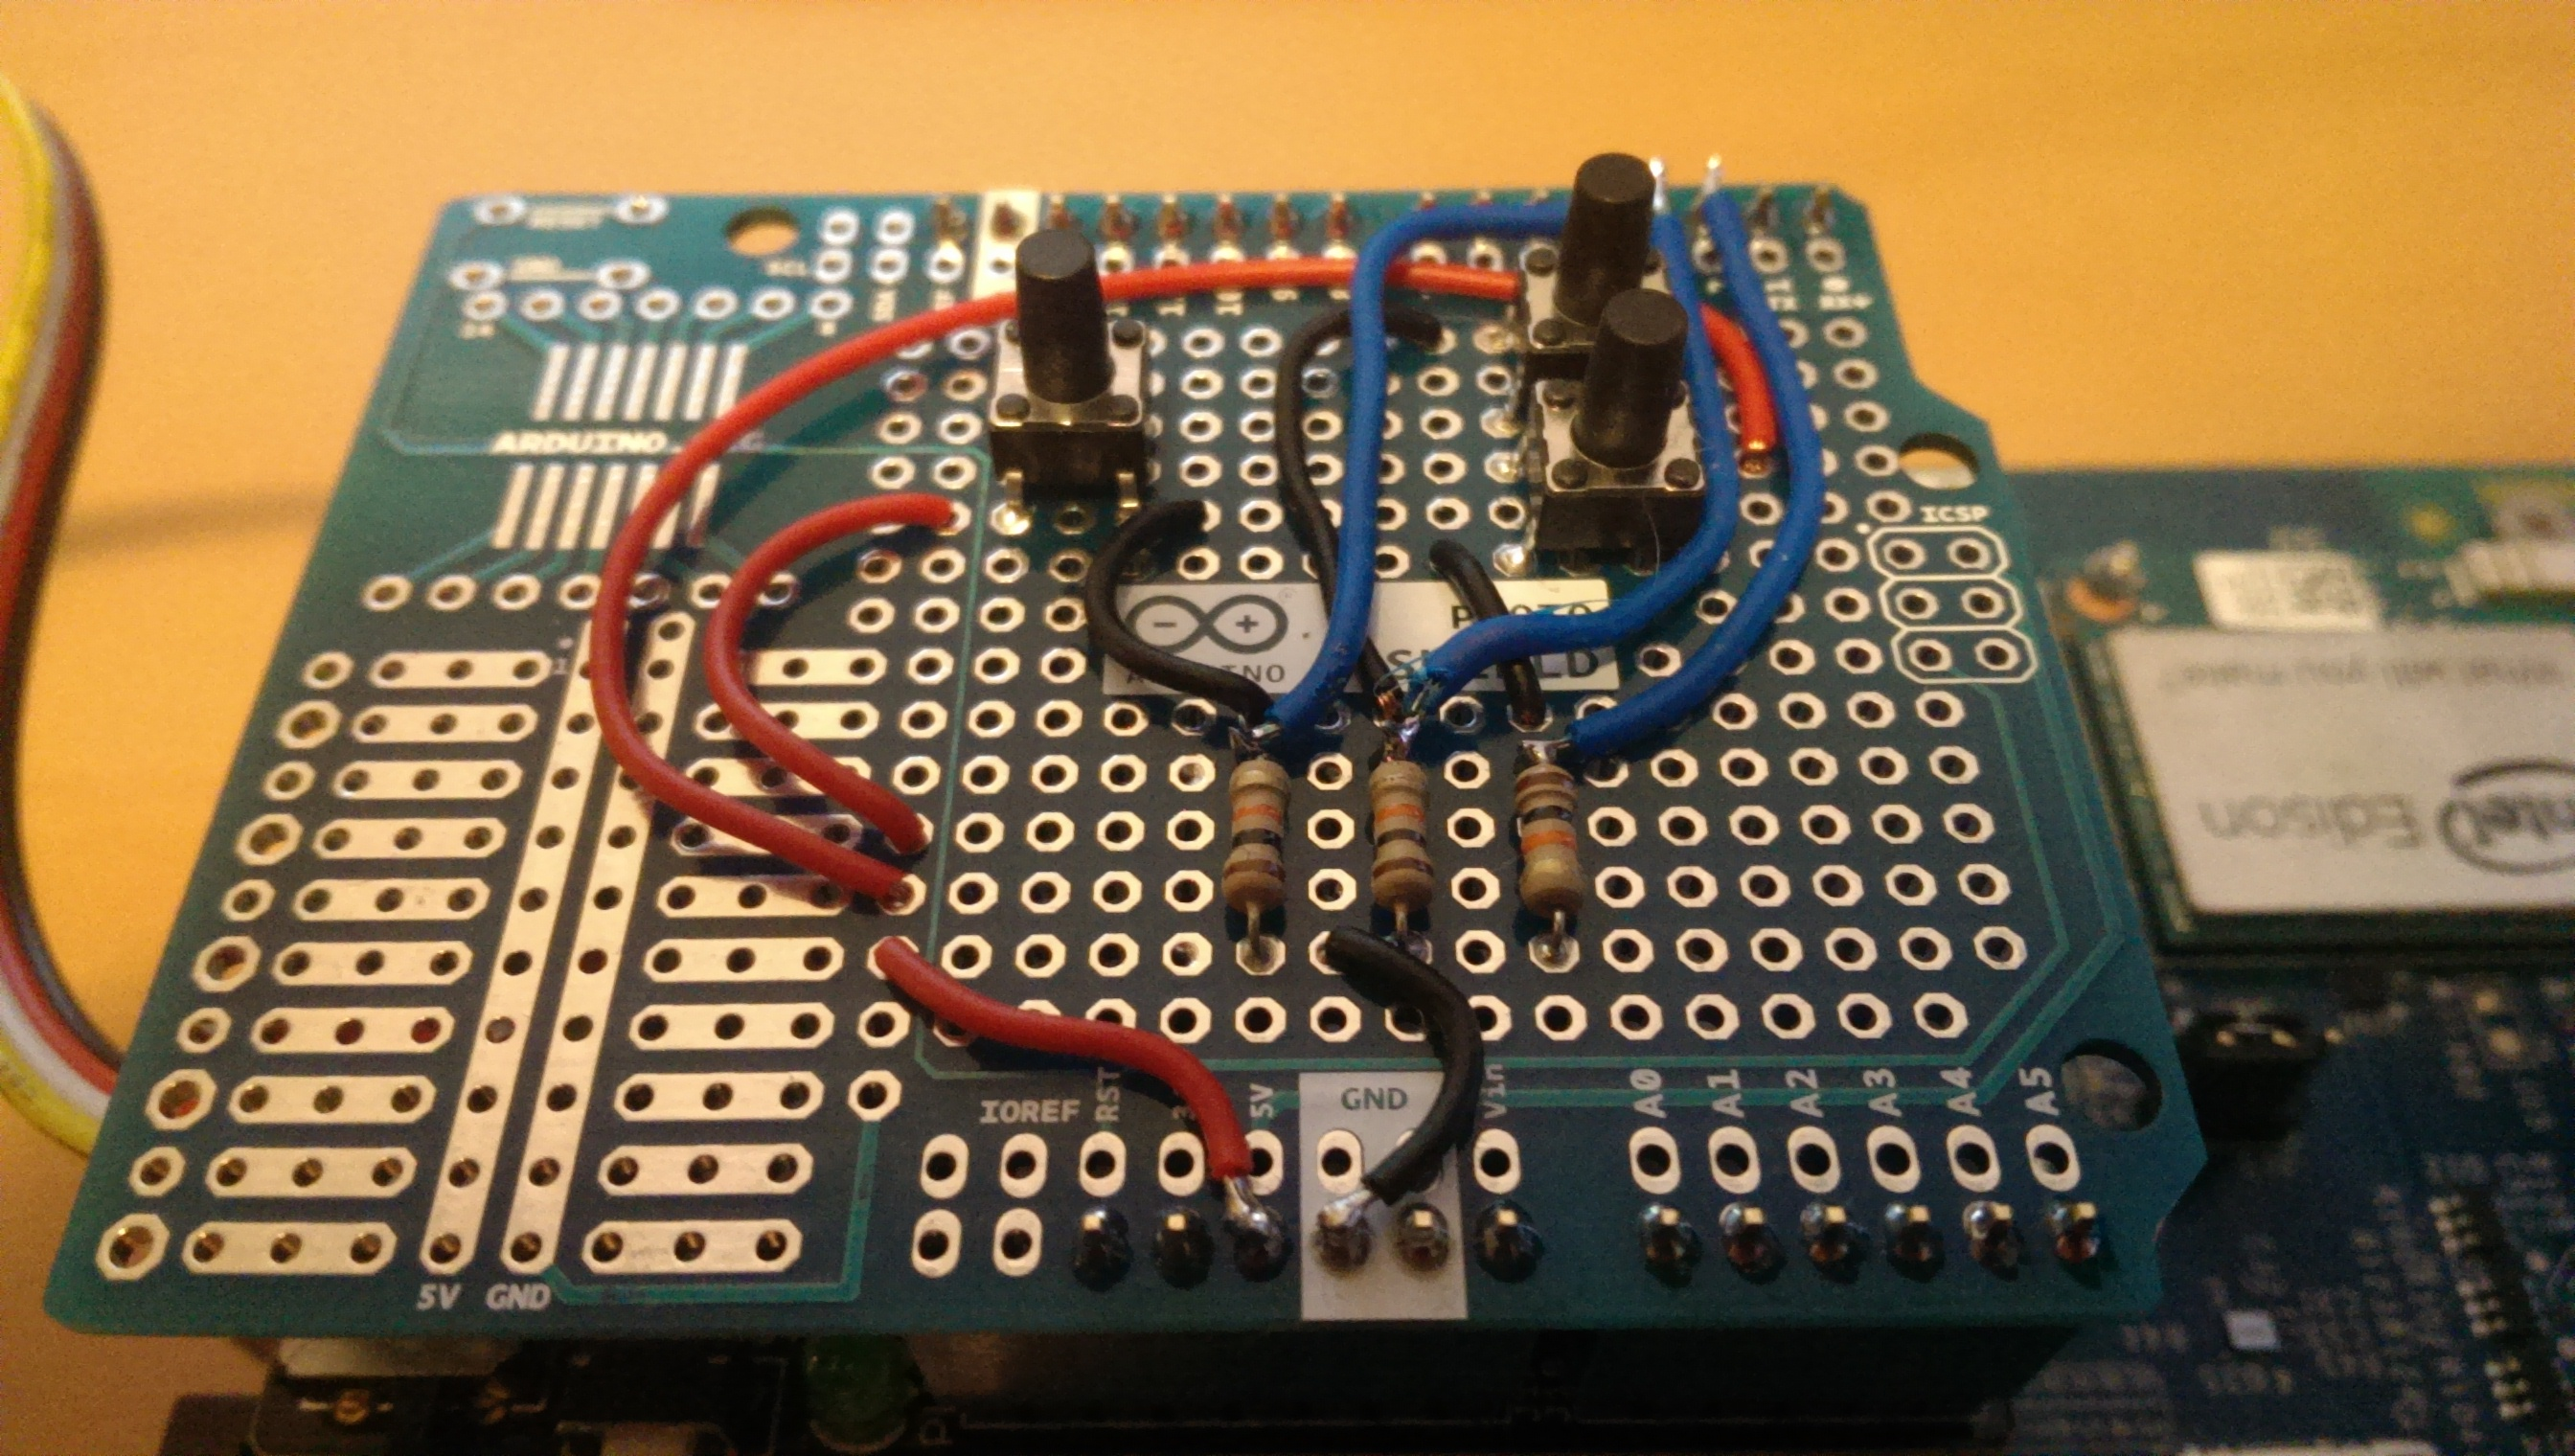
\includegraphics[width=300px]{images/buttons1}
	\caption{Buttons}
\end{figure}

The 3 pushbuttons are mounted on an Arduino proto shield and are "active-high" (this means 0V signal when the button is not pressed and 5V signal when the button is pressed).
Each button is connected to a digital pin on the arduino header (pin 2, pin 3 and pin 4).In my software I am configuring these pins as input pins. Furthermore interrupts are used to handle a button press.
I didn't implement any button debouncing in hardware, so I just added simple debouncing in software using a timer.

\begin{figure}[h]
	\includegraphics[width=300px]{images/LCD}
	\caption{LCD}
\end{figure}

The LCD I used is part of the Seeed Grove Starter Kit Plus. The LCD was connected to the Intel Edison Arduino board using the Grove base board.
Using the LCD in software is very easy , as the driver for this LCD is already in the Intel UPM repository.
The only thing I added is a very simple C++ wrapper for the existing C code.

\subsection{Statemachine}
The software now has code for audio playback and Bluetooth configuration and also code for the user interface(buttons and LCD), but we still need something to connect it all together.
The "statemachine" pattern is commonly used for this type of problem. I could have build a simple state machine in C++ direcly, but I decided to use the State Machine Compiler (\url{http://smc.sourceforge.net/}) instead. SMC allows me to make a clean seperation between the design of the state machine itself and the implementation in code. 
SMC basically compiles a statemachine design (in a  text file) to sourcecode in a number of languages (C++, Java, etc.). 
This also enables easy extensions of the sourcecode in the future.


\chapter{Conclusion}
The development of the E27radio was a bumpy road, but it works quite well in the end. I just had enough time to finish a first basic prototype of E27-radio in time for the contest and I already identified quite a few things that still need to be done :
\begin{itemize}
	\item Implement/improve exception handling in software 
	(currently only 'happy flow' is supported)
	\item Simplify setup procedure (currently the initial setup needs to be done via the command line , for example pairing the Intel Edison with a Bluetooth device).
	\item Implement extraction of metadata from Internet radio streams (for example title and artist for the current song)
	\item Volume control for the radio stream
\end{itemize}
I hope this project helps other people to build their own internet radio (or any other application for that matter). The Intel Edison is a good platform for building an internet radio, as it has Wifi, Bluetooth and enough processing power. The only disadvantage is that its limited graphical processing capablities make it more difficult to use a graphical LCD in the user interface for an Internet radio client.

\begin{appendices}

\chapter{About the author}
Jeroen Vennegoor op Nijhuis is a Dutch engineer. 
He lives in Eindhoven( the Netherlands) . He studied at the University of Twente and has a MSc degree in Mechanical Engineering. His professional interests and skills  range from mechanical design to electronics and software. His professional experience has been mostly in R\&D and the development of new products.\\
For more information:\\
LinkedIn: \url{https://nl.linkedin.com/in/jeroenvennegoor}

\end{appendices}


\end{document}